\documentclass[a4paper]{article}

%% Language and font encodings
\usepackage[spanish]{babel}
%\selectlanguage{spanish}
\usepackage[utf8x]{inputenc}
\usepackage[T1]{fontenc}
%% Sets page size and margins
\usepackage[a4paper,top=3cm,bottom=2cm,left=3cm,right=3cm,marginparwidth=1.75cm]{geometry}
\usepackage{graphicx}
\usepackage{titling}
\usepackage{amsmath}
\usepackage[toc,page]{appendix}
\usepackage{listings} % For matlab code
\usepackage[colorinlistoftodos]{todonotes}
\usepackage[colorlinks=true, allcolors=blue]{hyperref}
\usepackage{color} %red, green, blue, yellow, cyan, magenta, black, white
\definecolor{mygreen}{RGB}{28,172,0} % color values Red, Green, Blue
\definecolor{mylilas}{RGB}{170,55,241}

% Un poco jugado pero funciona
\title{\\[3cm]
\large Introducción a las Ciencias de la Tierra y el Espacio I\\[0.5cm]
Práctica 4\\[1cm]
\bf Análisis del ozono atmosférico}
\author{Juan Ramírez}

% Don't indent paragraphs
\setlength{\parindent}{0ex}
\setlength{\parskip}{1em}

\lstset{language=Matlab,%
    xleftmargin=.5in,
    basicstyle=\tiny,
    breaklines=true,%
    morekeywords={matlab2tikz},
    keywordstyle=\color{blue},%
    morekeywords=[2]{1}, keywordstyle=[2]{\color{black}},
    identifierstyle=\color{black},%
    stringstyle=\color{mylilas},
    commentstyle=\color{mygreen},%
    showstringspaces=false,%without this there will be a symbol in the places where there is a space
    numbers=left,%
    numberstyle={\tiny \color{black}},% size of the numbers
    numbersep=9pt, % this defines how far the numbers are from the text
    emph=[1]{for,end,break},emphstyle=[1]\color{red}, %some words to emphasise
    %emph=[2]{word1,word2}, emphstyle=[2]{style},    
}


\begin{document}

% Add title
\maketitle

% Put floating images (has to be after the title)
\usetikzlibrary{calc} % for picture positioning
% UdelaR - top left
\begin{tikzpicture}[remember picture,overlay]
 \node[anchor=north west,inner sep=0pt] at ($(current page.north west)+(2cm,-2cm)$) {
  
\includegraphics[width=2cm]{assets/udelar_v.png}
 };
\end{tikzpicture}
% Fcien - top right
\begin{tikzpicture}[remember picture,overlay]
 \node[anchor=north east,inner sep=0pt] at ($(current page.north east)+(-2cm,-2cm)$) {
  
\includegraphics[width=2cm]{assets/fcien_v.png}
 };
\end{tikzpicture}

\bigskip

\tableofcontents

\newpage
\section*{Introducción}

El objetivo de esta práctica es estudiar la evolución de las concentraciones de Ozono en la atmósfera en diferentes localidades y a lo largo de los años.

Empezaremos estudiando la variación en los niveles de ozono a lo largo del año en la Antártida para los años 2000 y 2005, para luego estudiar la variación anual del agujero de ozono entre 1978 a 2012. Finalmente, estudiaremos los niveles de ozono sobre Uruguay.

Nuestro estudio consistirá en el análisis de imágenes satelitales capturadas a lo largo de los años sobre el polo sur y el globo terráqueo.

Un ejemplo de dichas imágenes se puede observar en la Figura \ref{fig:sample}.

\begin{figure}[ht]
\centering
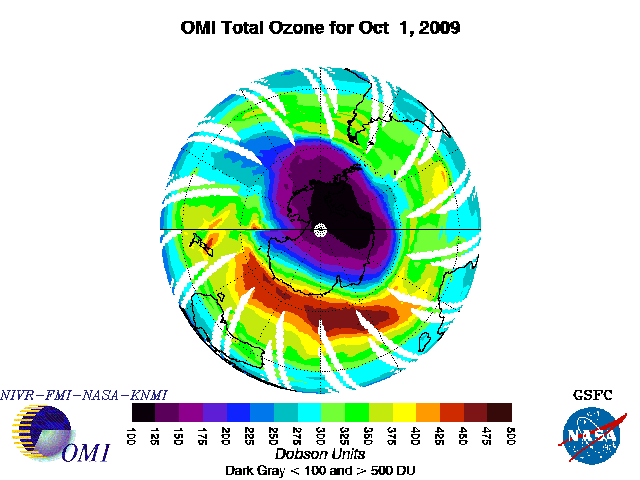
\includegraphics[width=0.9\textwidth]{assets/sample.png}
\caption{\label{fig:sample}Ejemplo de captura satelital.}
\end{figure}

Para la parte \hyperref[section:parte1]{1} y \hyperref[section:parte3]{3} de la práctica, se interpretará el valor correspondiente al color indicado en la escala de abajo, aumentando algún grado o disminuyendo en caso de haber superposición de colores.\\
Por ejemplo, si en una zona hay una combinación de azul oscuro (225) con azul claro (250), tomaremos el valor 235 o, si visualmente se notara una predominancia de azul oscuro, tomaríamos un valor más cercano a 225; de la misma manera, si el color dominante fuera el azul claro, tomaríamos un valor más cercano al 250.

\newpage
\section{Variaciones estacionales del agujero de ozono}
\label{section:parte1}

Este experimento consiste en estudiar visualmente las imágenes del Polo Sur generadas en los años 2000 y 2005 y, a partir de la escala definida en la imagen, extraer intuitivamente un número asociado al nivel de ozono correspondiente. Por ejemplo, en la Figura \ref{fig:sample}, la región negra corresponde a un nivel de ozono menor a 124 unidades Dobson [\ref{bib:letra}]. 

Los valores obtenidos a partir de esta observación se pueden ver en la Tabla \ref{table:parte1}.

No se tienen datos para los meses de Abril a Setiembre, esto se debe a que el satélite utiliza un espectrómetro de escaneo que recibe la luz reflejada por la superficie y atmósfera terrestre. En invierno el polo sur <<le da la espalda>> al sol, por lo que no refleja suficiente luz como para obtener una buena captura.

\begin{table}[ht]
\centering
\begin{tabular}{c | c | c}
Mes & Año 2000 & Año 2005 \\\hline
Enero & 265 & 275\\
Febrero & 275 & 260\\
Marzo & 275 & 250 \\
Abril & - & -\\
Mayo & - & -\\
Junio & - & -\\
Julio & - & -\\
Agosto & - & -\\  
Setiembre & - & -\\
Octubre & 100  & 100\\
Noviembre & 285 & 185\\
Diciembre & 310  & 225\\
\end{tabular}
\caption{\label{table:parte1}Niveles de ozono en el polo sur}
\end{table}

En la Figura apéndice \ref{appendix:year2000} se puede ver una miniatura de todas las tomas correspondientes al año 2000. Las zonas en blanco son las que no tienen datos, notar que esa zona se va agrandando a medida que avanza el invierno austral y empieza a achicarse con la llegada de la primavera.

Los niveles de ozono en el Polo Sur para los años 2000 y 2005 se ilustran en la Figura \ref{fig:ps2000y2005}.

\begin{figure}[h!]
\centering
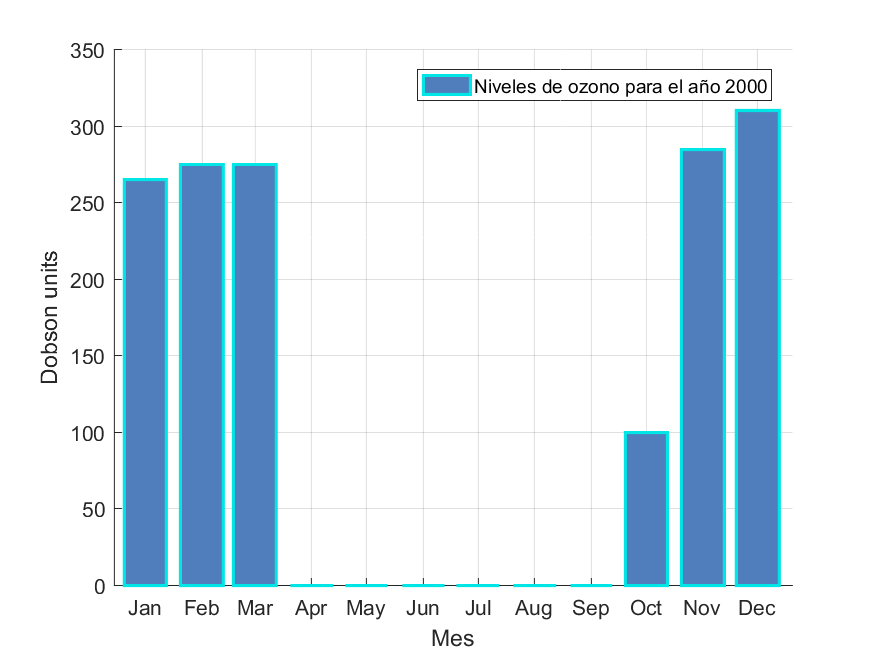
\includegraphics[width=0.45\textwidth]{assets/PS2000.png}
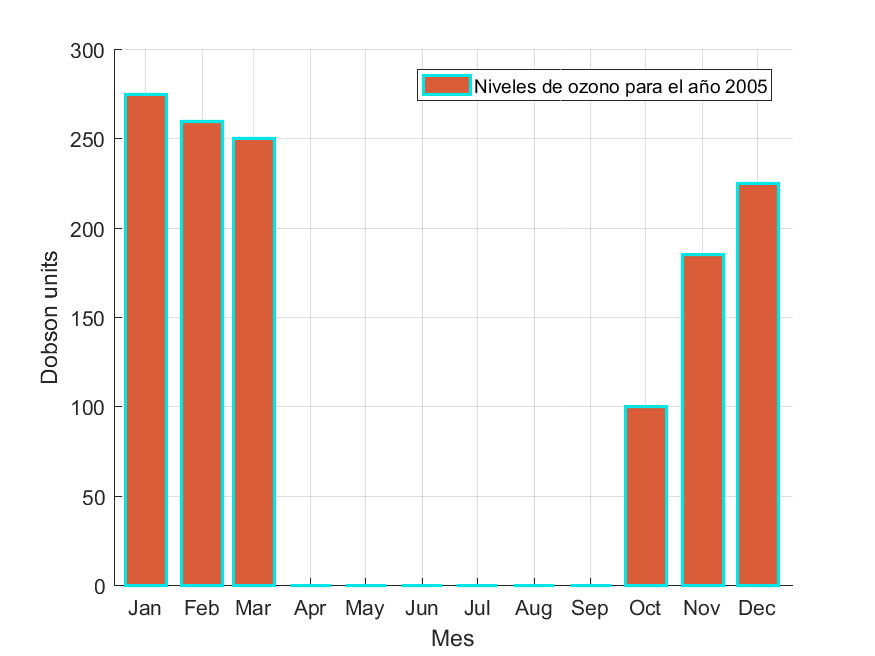
\includegraphics[width=0.45\textwidth]{assets/PS2005.png}
\caption{\label{fig:ps2000y2005}Niveles de ozono para los años 2000 y 2005}
\end{figure}

Una situación interesante (y preocupante) se hace presente al superponer ambas gráficas, pues se ve claramente que en el 2005 los niveles de ozono tienden a ser más bajos que en el 2000.

\begin{figure}[h!]
\centering
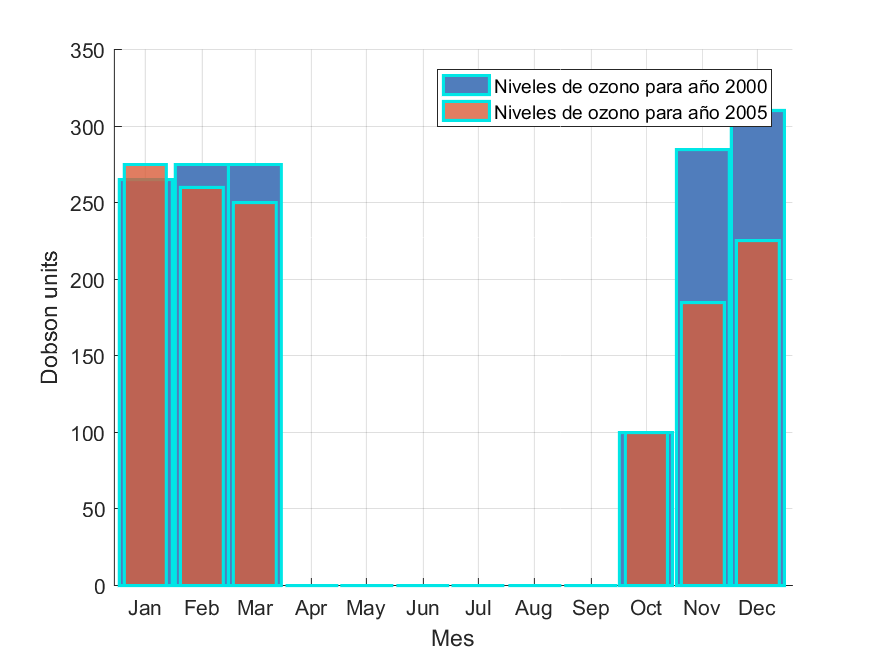
\includegraphics[width=0.9\textwidth]{assets/PS2000vs2005.png}
\caption{\label{fig:ps2000vs2005}Comparativa años 2000 y 2005}
\end{figure}

En el 2005 no solo es más bajo el nivel de ozono a nivel general sino que se nota que las recuperaciones son más lentas.

En cuanto a la información faltante entre Abril y Setiembre solo podemos especular que el nivel de ozono va bajando gradualmente hasta llegar a un punto mínimo entre Setiembre y Octubre, esto lo podemos inferir a partir de las imágenes que se pueden observar en el apéndice \ref{appendix:year2000}. Particularmente, en setiembre se observa (ver Figura \ref{fig:set2000})  que el nivel de ozono está por debajo de las 175 unidades Dobson en casi toda la Antártida.

\begin{figure}[h!]
\centering
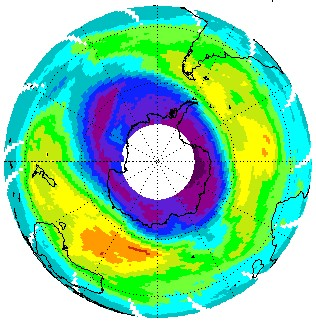
\includegraphics[width=0.5\textwidth]{assets/mini/09.jpg}
\caption{\label{fig:set2000}Setiembre de 2000}
\end{figure}

Finalmente, para comparar el tamaño del agujero de ozono entre ambos años, tomamos como muestra los meses de Setiembre y Octubre, notando que en ambos años se da que en Setiembre el agujero de ozono es más grande.

En la Figura \ref{fig:area2000vs2005} se puede observar el contorno del agujero de ozono dibujado con la herramienta \href{https://la.mathworks.com/help/images/ref/imfreehand.html}{imfreehand} de MATLAB.

Las áreas del agujero de ozono medidas para esos períodos son se pueden observar en la Tabla \ref{table:area2000vs2005} y en el apéndice \ref{appendix:calculoArea} se explica el método utilizado para calcular el área.

\begin{figure}[h!]
\centering
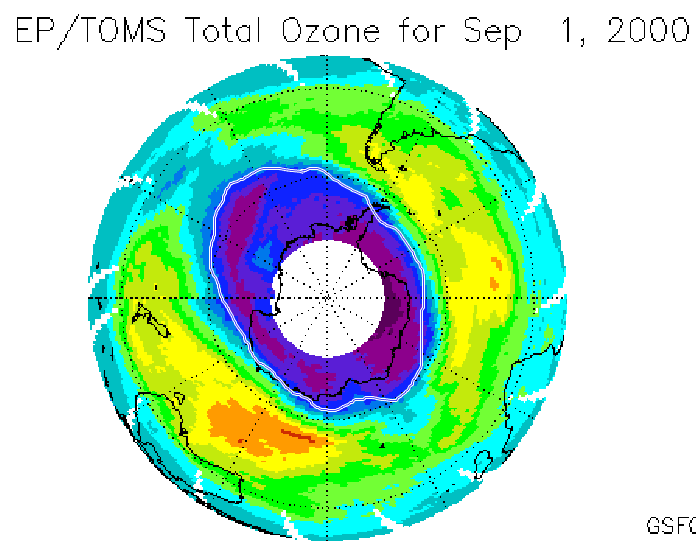
\includegraphics[width=0.4\textwidth]{assets/hole_set2000.png}
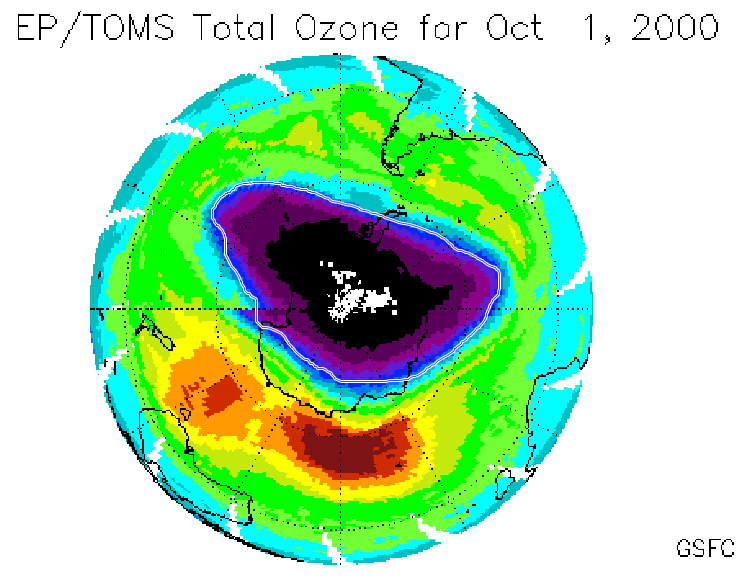
\includegraphics[width=0.4\textwidth]{assets/hole_oct2000.png}
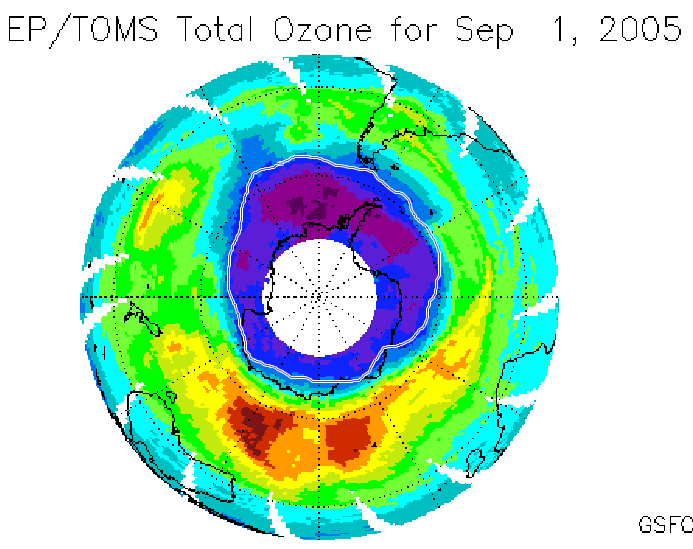
\includegraphics[width=0.4\textwidth]{assets/hole_set2005.png}
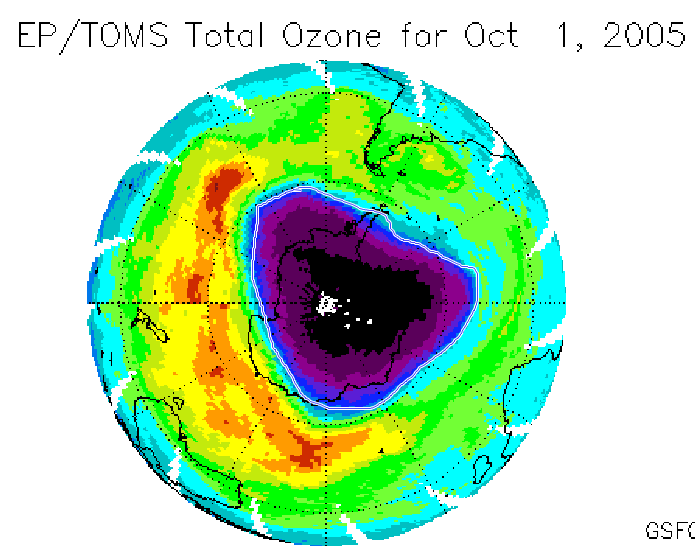
\includegraphics[width=0.4\textwidth]{assets/hole_oct2005.png}
\caption{\label{fig:area2000vs2005}Área del agujero de ozono en Setiembre y Octubre de 2000 y 2005}
\end{figure}

\bigskip

% Set 2000: 2.7731e+07
% Oct 2000: 2.4119e+07
% Set 2005: 2.6139e+07
% Oct 2005: 2.4483e+07
\begin{table}[h!]
\bigskip
\centering
\begin{tabular}{c | c | c}
Mes & Año 2000 & Año 2005 \\\hline
Setiembre & 27.7  & 24.1\\
Octubre & 26.1 & 24.4\\
\end{tabular}
\caption{\label{table:area2000vs2005}Área (en millones de $km^2$) del agujero de ozono}
\end{table}



\newpage
\section{Variación anual del tamaño del agujero de ozono}
\label{section:parte2}

En la Figura \ref{fig:variacionOzono} se muestra la variación del tamaño del agujero de ozono desde el año 1978 hasta el 2012. Con excepción del año 1995, del cual no tenemos datos.

\begin{figure}[ht]
\centering
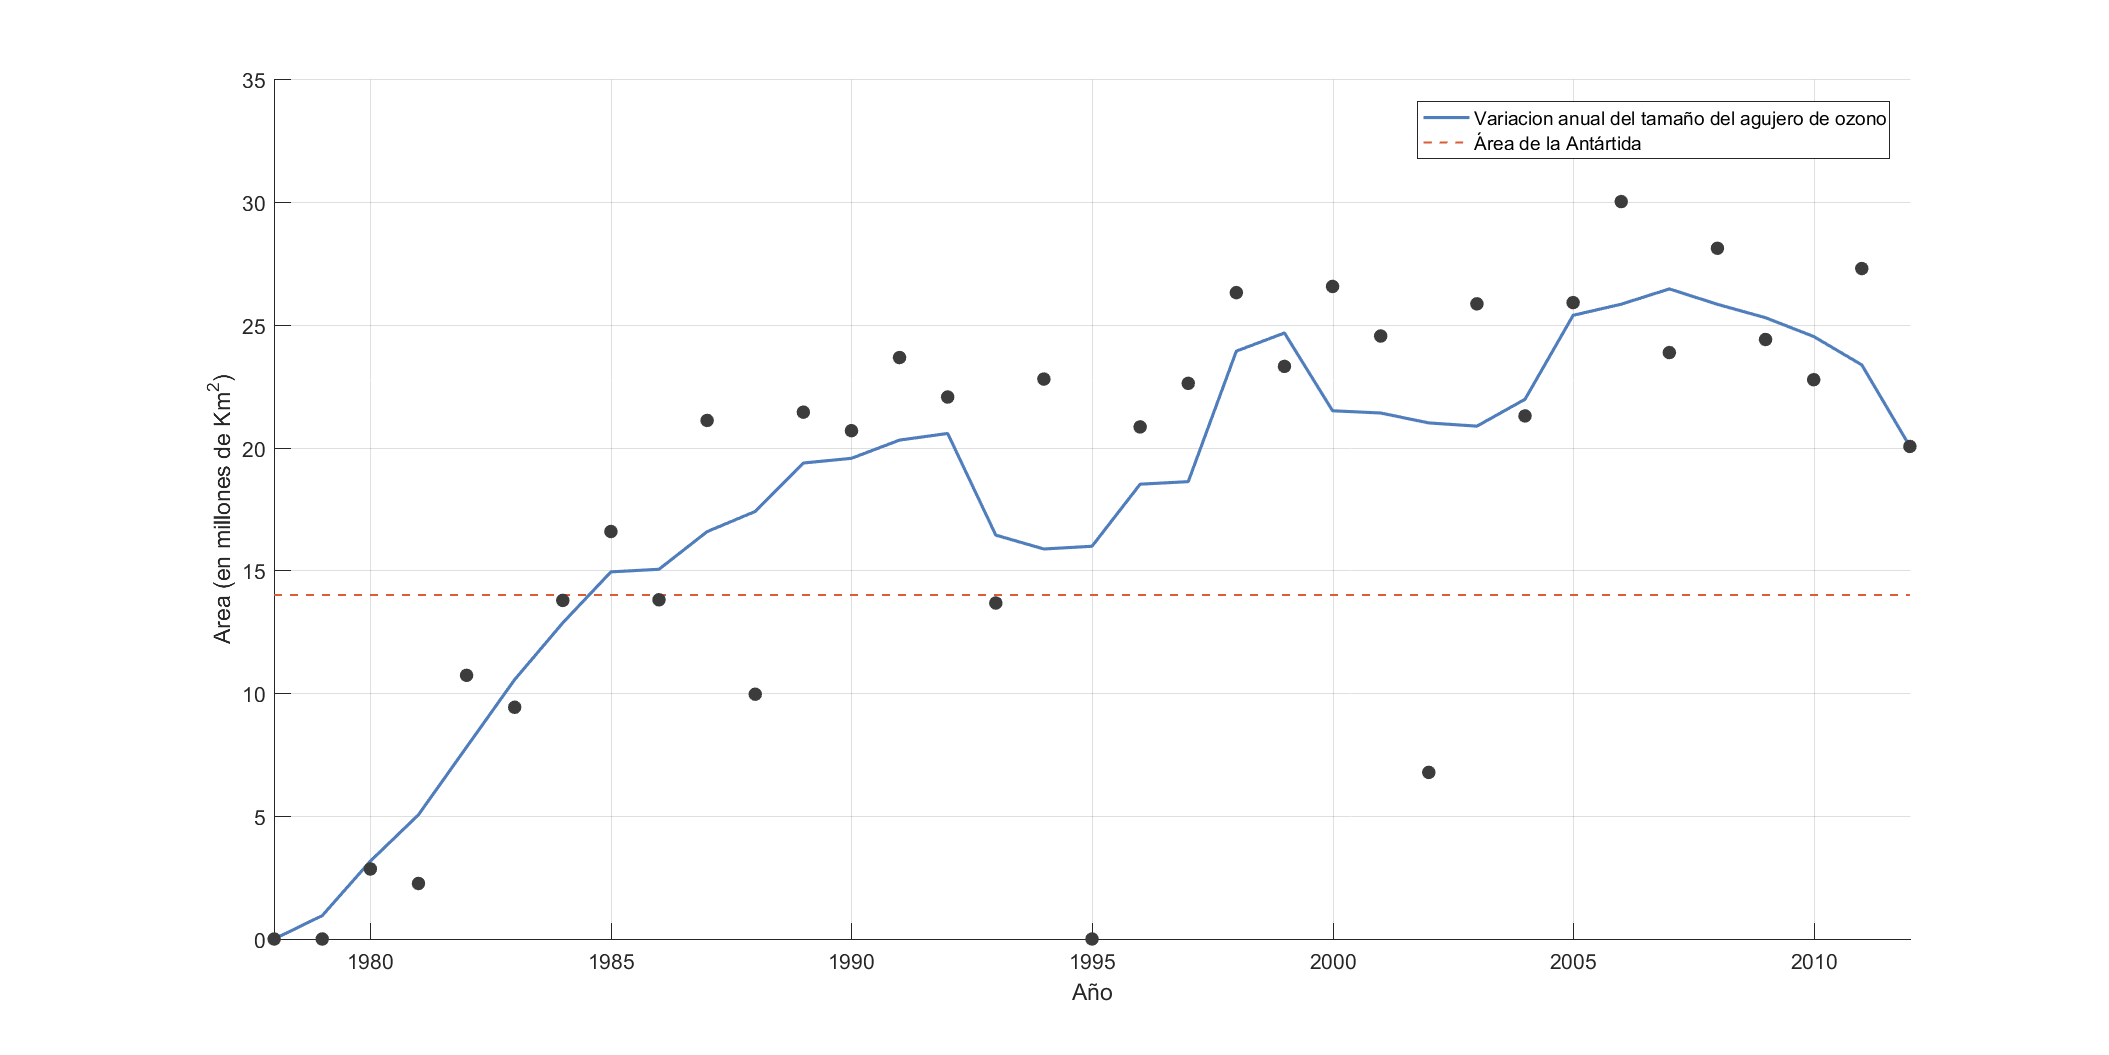
\includegraphics[width=1\textwidth]{assets/variacionOzono.png}
\caption{\label{fig:variacionOzono}Evolución del agujero de ozono a lo largo de los años}
\end{figure}

Ya en la mitad de la década de los 80 el agujero de ozono superaba el área de la Antártida y llegó a ser más del el doble de grande, teniendo un pico histórico en el año 2006. Luego se observa que el área ha ido bajando de forma muy lenta. Según un comunicado de la NASA [\ref{bib:nasaArticle}], el agujero de ozono alcanzó un mínimo histórico en 2017, cuando el 11 de Setiembre alcanzó un tamaño máximo de 12,123 millones de kilómetros cuadrados.

Comparando con los datos presentados en el anexo de la letra [\ref{bib:letra}], particularmente con la Figura 1 del Anexo 2, se concluye que los resultados medidos son muy similares y, además, los gráficos permiten reforzar las conclusiones realizadas en la sección anterior, donde estimábamos que Setiembre es el mes en el que se da el mínimo nivel de ozono atmosférico.

Sin embargo, se nota una discrepancia en el valor medido para el año 2002. Según nuestros datos el tamaño del agujero de ozono al 1ro de octubre de 2002 fue de unos 6.9 millones de kilómetros cuadrados, algo que se corresponde con el mínimo medido ese año. Para responder este enigma corresponde revisar la figura siguiente (ver Figura \ref{fig:letra_fig2}), donde (en verde) se observa la variación del área para dicho año y se ve que en octubre ya había alcanzado su mínimo.

\begin{figure}[ht]
\centering
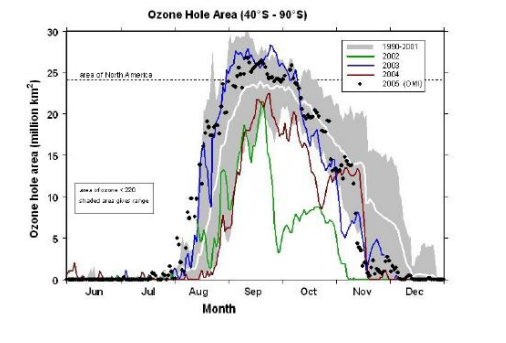
\includegraphics[width=0.7\textwidth]{assets/letra_fig2.png}
\caption{\label{fig:letra_fig2}Figura 2 Anexo 2 (letra)}
\end{figure}

En el apéndice \ref{appendix:calculoArea} se explica la metodología utilizada para calcular el área.

\newpage
\section{Niveles de ozono sobre Uruguay}
\label{section:parte3}

Se estudia la evolución en los niveles de ozono en Uruguay para el año 2005. Los datos obtenidos se muestran en la Tabla \ref{table:uy2005}

\begin{table}[ht]
\centering
\begin{tabular}{c | c}
Mes & Niveles de ozono \\\hline
Enero & 275\\
Febrero & 240\\
Marzo & 285 \\
Abril & 275\\
Mayo & 275\\
Junio & 295\\
Julio & 280\\
Agosto & 315\\  
Setiembre & 340\\
Octubre & 310\\
Noviembre & 320\\
Diciembre  & 280\\
\end{tabular}
\caption{\label{table:uy2005}Niveles de ozono en Uruguay para el año 2005}
\end{table}


TODO: Continuar acá

\begin{figure}[ht]
\centering
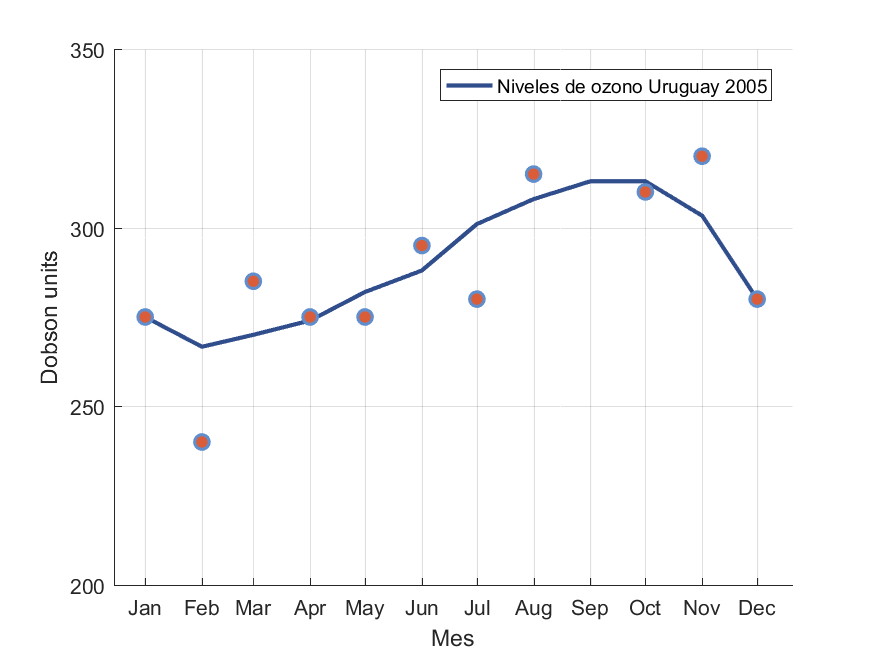
\includegraphics[width=0.8\textwidth]{assets/UY2005.png}
\caption{\label{fig:area_antartida}Niveles de ozono en Uruguay para el año 2005}
\end{figure}
          

\newpage
\begin{appendices}

\section{Tomas satelitales del Polo Sur correspondientes al año 2000}
\label{appendix:year2000}

\begin{figure}[ht]
\centering
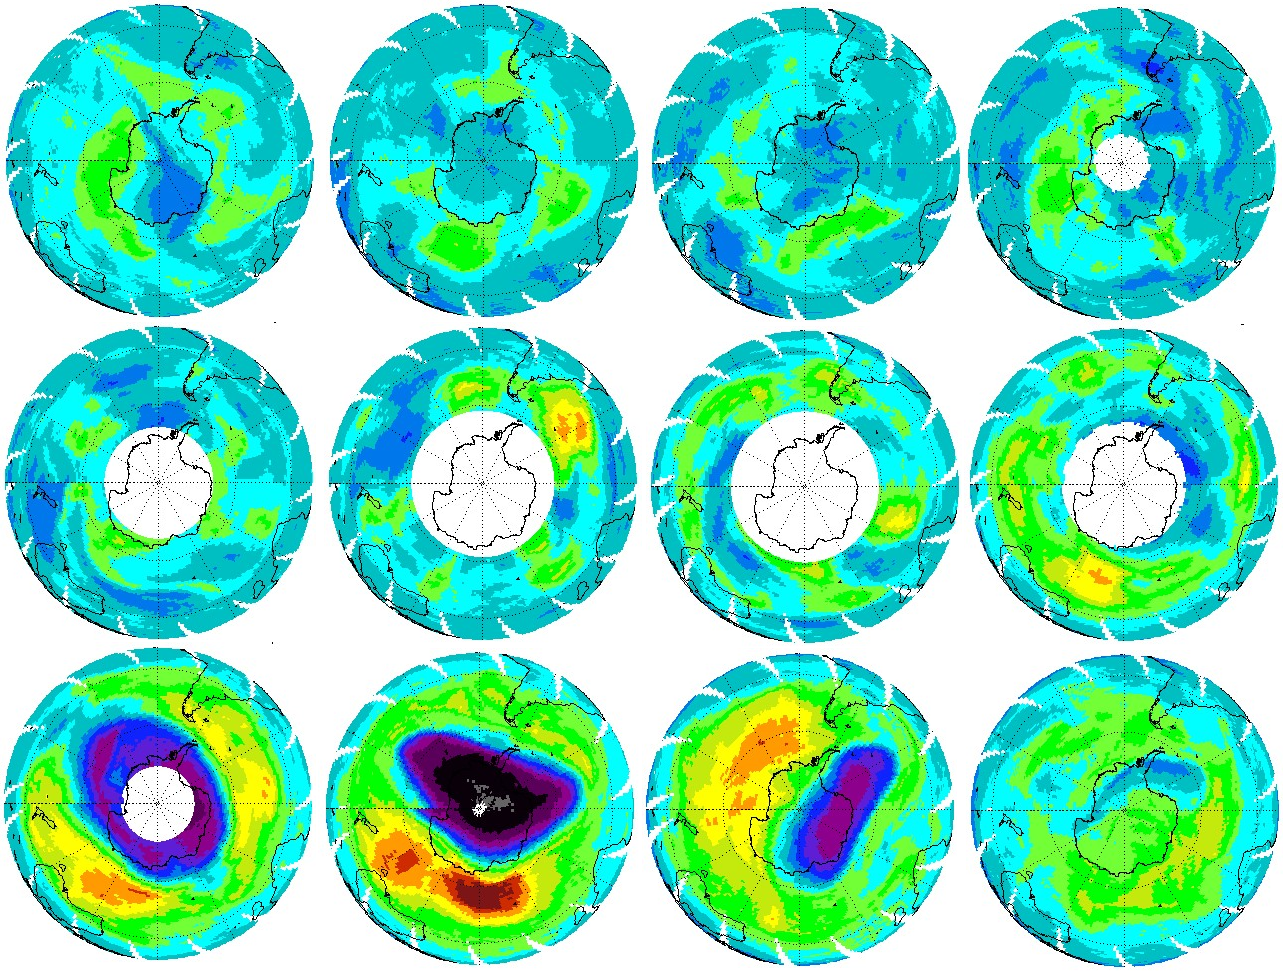
\includegraphics[width=0.99\textwidth]{assets/year2000.png}
\caption{\label{fig:year2000}Capturas satelitales desde Enero a Diciembre de 2000}
\end{figure}

\section{Sobre el cálculo del área}
\label{appendix:calculoArea}

Para calcular el área en $km^2$ se tomó el área de un terreno conocido para interpolar. En este caso, dato que él área de la Antártida es conocida (14 millones de $km^2$) se tomó midió el área de la Antártida utilizando \href{https://la.mathworks.com/help/images/ref/imfreehand.html}{imfreehand} sobre una de las imágenes, de la siguiente manera:

\begin{lstlisting}
h = imfreehand;
pos = getPosition(h);
close all;
area = polyarea(pos(:,1), pos(:,2));
\end{lstlisting}

En la Figura \ref{fig:area_antartida} se puede observar la región dibujada. Luego, se calculó el área utilizando la función \href{https://la.mathworks.com/help/images/ref/polyarea.html}{polyarea} y, finalmente, se computó la escala.

\begin{figure}[ht]
\centering
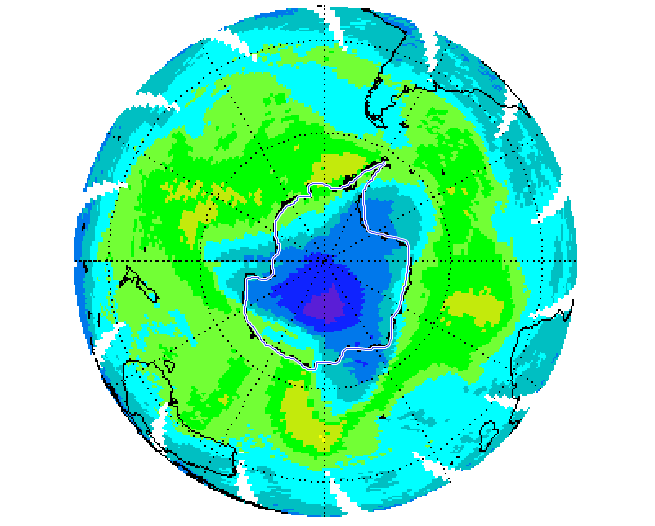
\includegraphics[width=0.8\textwidth]{assets/area_antartida.png}
\caption{\label{fig:area_antartida}Área de la Antártida}
\end{figure}

El resultado de la medición fue $8.0966 \times 10^3$ (píxeles cuadrados), considerando que el área real de la Antártida, la escala queda definida por $\frac{14 \times 10^6}{8.0966 \times 10^3} = 1.7291 \times 10^3$.




\section{Script blah.m}
\label{appendix:B}

Script utilizado para el experimento N° 2.

%\lstinputlisting{assets/stefan_boltzmann.m}
%\lstinputlisting{assets/udelar_v.m}



\end{appendices}

\begin{thebibliography}{9}
\bibitem{practica3}\label{bib:letra}
  Instituto de Física - Facultad de Ciencias,
  \emph{Letra de la práctica 4 - Introducción a las Ciencias de la Tierra y el Espacio I},
  Online at https://bit.ly/2JsnaxP
\bibitem{practica3}\label{bib:nasaArticle}
  Katy Mersmann - NASA's Earth Science News Team & Theo Stein - NOAA Office of Oceanic and Atmospheric Research, Boulder, Co.,
  \emph{Warm Air Helped Make 2017 Ozone Hole Smallest Since 1988},
  Online at https://go.nasa.gov/2sAw3eZ
\end{thebibliography}

\end{document}
